
The standard $k$-median problem attempts to open a facility set which optimizes global welfare by minimizing the average travel time per person, or equivalently, the total travel time of all people. One concern is that if a small percentage of the population were located in difficult-to-reach areas, it might skew the set of facilities opened in a way that significantly lowers the global quality of the solution. This effect can be very dramatic in the $k$-supplier problem, where one bad client can single-handedly force a hospital to be opened in an otherwise unhelpful location. 

Consider the following simple example. Suppose the population exists in a single, tight cluster, except for one client who lives 30km away. Also suppose we may only open one facility.  However, the optimal solution to $k$-supplier will prefer a location halfway between the tight population cluster and the single client, such that all clients have to travel 15km. This is the most fair solution in the $k$-supplier sense, but it would be much more beneficial globally to open the facility within the tight cluster, so that most clients are extremely close, and only one client must travel 30km. 

If we are allowed to ignore a small number of people, can the average connection cost of the remaining population be significantly improved? To explore this question we develop two modified formulations of the $k$-median problem. These formulations address the following two questions. First, how well does the $k$-median solution do at minimizing the travel time of some fraction of the population of the population? Secondly, how well does the $k$-median solution do at maximizing the amount of people which obtain a specific travel time? Next, we will consider these formulations.

\subsubsection*{Minimizing cost of closest clients}
Given a cutoff distance $D$ and fraction $\epsilon$, we want to minimize the average cost of the closest $(1-\epsilon)n$ clients subject to the constraint that those clients are all within distance $D$ of an open facility. This is explicitly captured by the following program.

  \begin{alignat}{2}
   \text{LP1}: \text{min }   &  \sum_{i \in H, j \in P: w_{ij} \leq D} p_j d_{ij} x_{ij} \nonumber \\
    \text{s.t.} & \sum_{i \in H: w_{ij} \leq D} x_{ij} \leq 1    &\ & \forall j \in P \\
                             &  x_{ij} \leq y_i      & & \forall i \in H, j \in P: w_{ij} \leq D \\
                             & \sum_{i \in H} y_i \leq k\\                                                          %& \sum_{j \in P} p_j\left(1 - \sum_{i \in H: w_{ij} \leq D} x_{ij} \right) \leq  \epsilon \left( \sum_{j \in P}p_j \right) \\
& \sum_{j \in P} \sum_{i \in H: w_{ij} \leq D} p_j x_{ij} \geq  (1-\epsilon) \left( \sum_{j \in P}p_j \right) \\
&x_{ij}, y_i \in[0,1] &\qquad & \forall i\in H, j\in P
  \end{alignat}


We observe in Figure \ref{fig:kmed_vs_LP1} that our integral solutions to LP1 only marginally improve the travel time of the top $(1-\epsilon)n$ clients over that of the ordinary $k$-median solution. Since solving the LP1 formulation in integer form is NP-hard, we cannot tell for sure if there exist solutions which perform closer to the theoretical minimum given by the fractional LP solution. However, if our solutions are close to optimal, these results indicate that on real datasets, the ordinary $k$-median solution is already quite good with respect to the LP1 optimization criteria. It is not necessary to choose some parameters $D$ and $\epsilon$ and find a solution which specifically satisfies these. As long as $k$ is large enough, the ordinary $k$-median solution already performs quite well.

\subsubsection{Maximizing number of close clients}

%For $i\in H$ and $j\in P$, let $x_{ij}$ be an indicator for population node $j$ being assigned to a hospital at $i$, and let $w_{ij}$ be the cost of such an assignment. Let $y_i$ be an indicator for a hospital being opened at location $i\in H$. Let $k$ denote the number of hospitals, and $D$ denote the {\emph ideal} maximum cost for any client. 

In this formulation, we suppose we have fixed some acceptable travel cost $D$, and wish to maximize the number of clients which have a hospital within that distance. 




\begin{alignat}{2}
\text{LP2: max}  &\sum_{j\in P}\sum_{i\in H} x_{ij}p_j  && \nonumber\\
\label{eqn:violationsA1}
\text{s.t. } &x_{ij} \leq y_i &\qquad & \forall i\in H, j\in P\\
\label{eqn:violationsA2}
& x_{ij} = 0 &\qquad & \forall i\in H, j\in P \mbox{ with }d_{ij}>D\\
\label{eqn:violationsA3}
& \sum_{i\in H} x_{ij} \le 1  &\qquad & \forall j\in P\\
\label{eqn:violationsA4}
&\sum_i y_i \leq k\\
\label{eqn:violationsA5}
&x_{ij}, y_i \in[0,1] &\qquad & \forall i\in H, j\in P
\end{alignat}

We solve this formulation for $D$ varying from 2 to 7 hours, using $k=16$. We then take the solution to ordinary $k$-medain for $k=16$, and measure how many clients lie within distance $D$ for each value. The values are compared in Figure \ref{fig:LP2_AB}. 

\begin{figure}[h]
  \centering % left bottom right top
    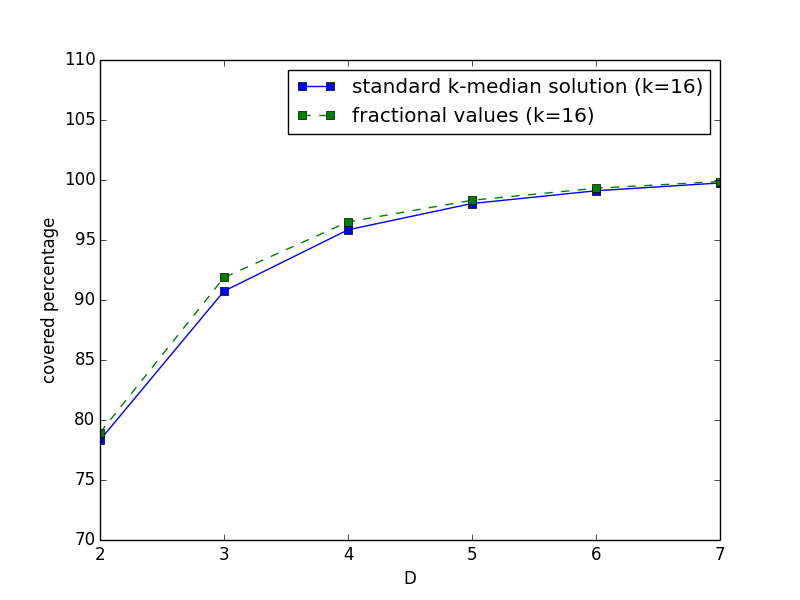
\includegraphics[width=0.4\textwidth]{figs/plotA16_min_violation.png}
	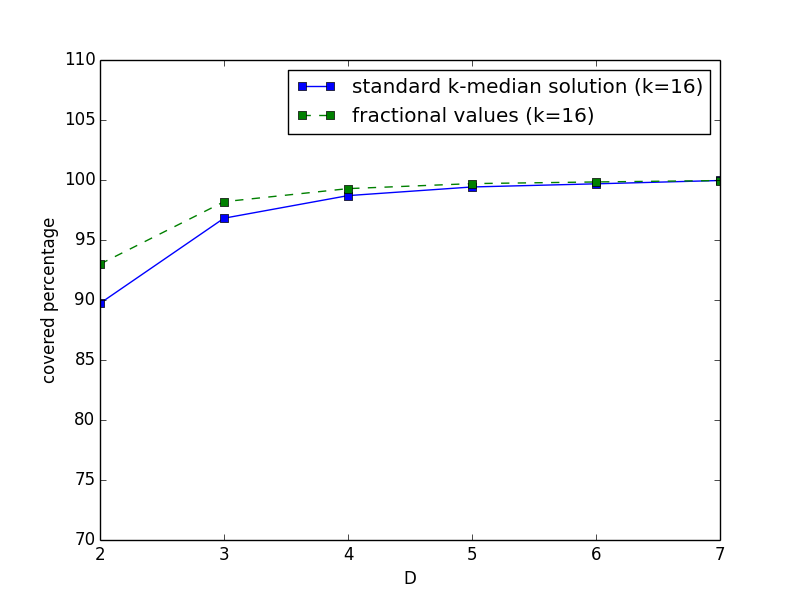
\includegraphics[width=0.4\textwidth]{figs/plotB16_min_violation.png}
\caption{Our results of solving LP2 for Dataset A (left), and B (right). (Liberia)} 
	\label{fig:LP2_AB}
\end{figure}

Figure \ref{fig:LP2_AB} shows that the $k$-median solution comes quite close to the fractional solution to LP2, which upper bounds the optimal integral solution to LP2. These results again suggest that the $k$-median solution is already quite robust, in that it already does a good job maximizing the number of clients within distance $D$, for many values of $D$ simultaneously. 

Our conclusion in this subsection is that it is only marginally beneficial to exclude any of the population as outliers. The ordinary $k$-median problem already yields a good quality solution. 

